\section{Balancing a search tree}
\label{sec:balancing_a_search_tree}

\begin{frame}
	\frametitle{It's all about balance}
	\begin{center}
		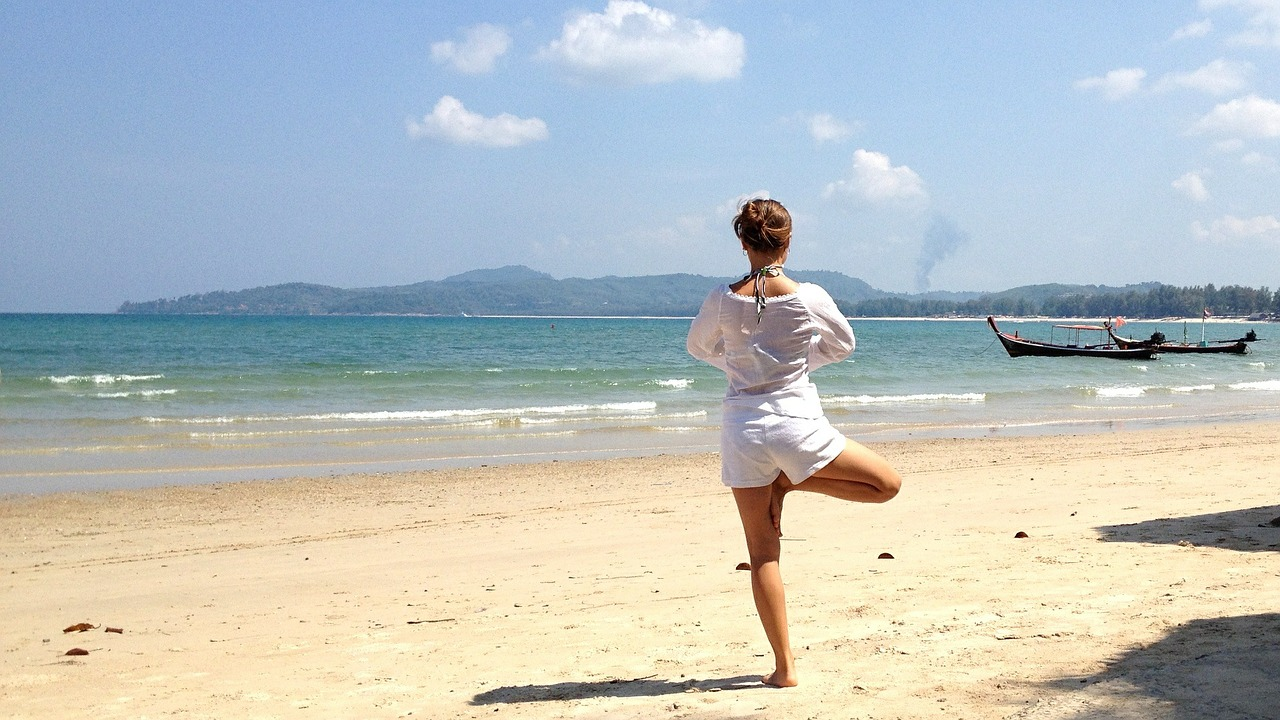
\includegraphics[width=0.8\textwidth]{figures/balance.jpg}\\
		\hspace*{15pt}\hbox{\scriptsize Image By:\thinspace{\itshape Evitaochel}}
		% https://pixabay.com/photos/balance-yoga-zen-exercise-405513/
	\end{center}
\end{frame}

\begin{frame}
	\frametitle{Limiting the height}
	\begin{block}{The idea}
		If we can somehow limit the height to be $\Theta(\log n)$ we are all set.
	\end{block}	
	\pause
	This is where the tens of options come in...
	\begin{itemize}
		\item AVL-trees
		\item Red-Black trees
		\item Splay-trees
		\item And many more\dots
	\end{itemize}
\end{frame}

\begin{frame}
	\frametitle{AVL-Trees}
	\framesubtitle{Named after Adel'son-Vel'skii and Landis}

		\begin{block}{AVL-trees}
			It is a binary search tree, with one more constraint:\\
			The height of the left-subtree and right-subtree of a node differ by at most 1 for all nodes in the tree.
		\end{block}	

	\begin{columns}
		\column{0.455\textwidth}

		\begin{tikzpicture}[
			level distance = 2.5em,
			level 1/.style={sibling distance=9em},
			level 2/.style={sibling distance=4.5em},
			level 3/.style={sibling distance=2.25em},
			]
			\node[ellipse] (t1) {12}
			child { node[ellipse]   {3}
				child[draw=white] { }
				child { node[ellipse] {9}}
			}
			child { node[ellipse]   {25}
				child { node[ellipse] {14}}
				child { node[ellipse] {29}
					child { node[ellipse] {26}}
					child { node[ellipse] {32}}
				}
			};
		\end{tikzpicture}
		\column{0.455\textwidth}

		\begin{questionblock}{Is it full?}
			Is this tree an AVL-tree?
		\end{questionblock}
		\pause
		\begin{answerblock}{}
			Yes :)	
		\end{answerblock}
	\end{columns}
\end{frame}

\begin{frame}
	\frametitle{AVL-trees}
	\begin{block}{Height}
		This guarantees the height to be $\Theta(\log n)$ (check the book for a proof if you want).
	\end{block}

	\pause
	\begin{problemblock}{Inserting/deleting nodes}
		How do we now insert or delete nodes from this AVL tree?
	\end{problemblock}
\end{frame}

\begin{frame}
	\frametitle{Inserting items}

	\begin{block}{Observations}
		\begin{itemize}
			\item If we insert like we did in a ``regular'' binary search tree\dots
			\item Then we only upset (potentially) the ancestors of the node where we insert it.
				\pause
			\item Let's look at an example ;)
		\end{itemize}
	\end{block}	
	\pause
	\begin{exampleblock}{Inserting an item}
		\begin{columns}
			\column{0.455\textwidth}

			\begin{tikzpicture}[
				level distance = 2.5em,
				level 1/.style={sibling distance=9em},
				level 2/.style={sibling distance=4.5em},
				level 3/.style={sibling distance=2.25em},
				scale=0.8,transform shape
				]
				\node[ellipse,onslide=<4>{draw=red}] (t1) {12}
				child { node[ellipse]   {3}
					child[draw=white] { }
					child { node[ellipse] {9}}
				}
				child { node[ellipse,onslide=<4>{draw=red},onslide=<5>{draw=blue}]   {\alt<6>{\color{blue}26}{25}}
					child { node[ellipse] {\alt<6>{\color{blue}{25}}{14}}
						child[onslide=<-5>{draw=white}] { node[ellipse] {\alt<6>{\color{blue}{14}}{}}}
						child[draw=white] { }
					}
					child { node[ellipse,onslide=<5>{draw=blue}] {29}
						child { node[ellipse,onslide=<5>{draw=blue}] {\alt<6>{\color{blue}27}{26}}
							child[draw=white] { }
							child[onslide=<6>{draw=white}] { node[ellipse] {\alt<6>{}{27}}}
						}
						child { node[ellipse] {32}}
					}
				};
			\end{tikzpicture}
			\column{0.455\textwidth}
			\begin{itemize}
				\item Two items are now upsetting the AVL-property.
					\pause
				\item So we need to fix that!
					\pause
				\item We can do so by \textit{rotating} some nodes around.
					\pause
				\item To end up with this.
			\end{itemize}
		\end{columns}
	\end{exampleblock}	
\end{frame}

\begin{frame}
	\frametitle{A tri-node restructering}
	\framesubtitle{Draw this for yourself!}
	\vspace{-15pt}
	\begin{columns}
		\column{0.455\textwidth}
			\begin{tikzpicture}[
				level distance = 2.5em,
				level 1/.style={sibling distance=9em},
				level 2/.style={sibling distance=5.5em},
				level 3/.style={sibling distance=4.5em},
				child anchor =north
				]
				\node[ellipse] (t1) {z}
				child { node[draw=black, regular polygon,regular polygon sides=3,anchor = north]   {T1}
				}
				child { node[ellipse]   {y}
					child { node[ellipse] {x}
						child { node[ellipse, regular polygon,regular polygon sides=3,anchor = north, draw=black] {T2}}
						child { node[ellipse, regular polygon,regular polygon sides=3,anchor = north, draw=black] {T3}}
					}
					child { node[ellipse, regular polygon,regular polygon sides=3,anchor = north, draw=black] {T4}
					}
				};
			\end{tikzpicture}
		\column{0.455\textwidth}
		\begin{itemize}
			\item This is the situation before inserting (we chose these heights to make the insertion interesting).
				\pause
				\begin{itemize}
					\item $z$ has a height of $h+2$
					\item $y$ has a height of $h+1$
					\item $x$ has a height of $h$
					\item $T1,T4$ have a height of $h$
					\item $T2,T3$ have a height of $h-1$
				\end{itemize}
				\pause
			\item We now insert an item into T3, which causes an imbalance in node z.
				\pause
				\begin{itemize}
					\item $z$ has a height of $h+3$
					\item $y$ has a height of $h+2$
					\item $x$ has a height of $h+1$
					\item $T1,T3,T4$ have a height of $h$
					\item $T2$ has a height of $h-1$
				\end{itemize}
		\end{itemize}
			
	\end{columns}
\end{frame}

\begin{frame}
	\frametitle{A tri-node restructering}
	\framesubtitle{Draw this for yourself!}
	\vspace{-15pt}
	\begin{columns}
		\column{0.455\textwidth}
			\begin{tikzpicture}[
				level distance = 2.5em,
				level 1/.style={sibling distance=9.5em},
				level 2/.style={sibling distance=5.0em},
				child anchor =north
				]
				\node[ellipse] (t1) {x}
				child { node[ellipse]   {z}
					child { node[draw=black, regular polygon,regular polygon sides=3,anchor = north]   {T1}
					}
					child { node[draw=black, regular polygon,regular polygon sides=3,anchor = north]   {T2}
					}
			}
				child { node[ellipse]   {y}
					child { node[ellipse, regular polygon,regular polygon sides=3,anchor = north, draw=black] {T3}}
					child { node[ellipse, regular polygon,regular polygon sides=3,anchor = north, draw=black] {T4}
					}
				};
			\end{tikzpicture}
		\column{0.455\textwidth}
		\begin{itemize}
			\item We can now rotate some stuff around :)
			\item Notice that the subtrees have not changed.
				\begin{itemize}
					\item $T1,T3,T4$ have a height of $h$
					\item $T2$ has a height of $h-1$
						\pause
					\item $z$ now has a height of $h+1$
					\item $y$ now has a height of $h+1$
					\item $x$ now has a height of $h+2$
				\end{itemize}
		\end{itemize}
			
	\end{columns}

	
\end{frame}

\begin{frame}
	\frametitle{Let's help ourselves}
	\begin{columns}
		\column{0.455\textwidth}
			
			\begin{tikzpicture}[
				level distance = 2.5em,
				level 1/.style={sibling distance=9em},
				level 2/.style={sibling distance=4.5em},
				level 3/.style={sibling distance=3em},
				level 4/.style={sibling distance=2em},
				]
				\node[ellipse] (t1) {12}
				child { node[ellipse]   {3}
					child { node[ellipse] {$\square$} }
					child { node[ellipse] {9}
						child { node[ellipse] {$\square$} }
						child { node[ellipse] {$\square$} }
					}
				}
				child { node[ellipse]   {25}
					child { node[ellipse] {14}
						child { node[ellipse] {$\square$} }
						child { node[ellipse] {$\square$} }
					}
					child { node[ellipse] {29}
						child { node[ellipse] {26}
							child { node[ellipse] {$\square$} }
							child { node[ellipse] {27}}
						}
						child { node[ellipse] {32}
							child { node[ellipse] {$\square$} }
							child { node[ellipse] {$\square$} }
						}
					}
				};
			\end{tikzpicture}
		\column{0.455\textwidth}
		\begin{itemize}
			\item Let's draw the non-existing leafs!
			\item This will help us identify what to rotate :)
				\pause
			\item And let's do this on the board.
		\end{itemize}
	\end{columns}
\end{frame}

\begin{frame}
	\frametitle{Phew...}
	\begin{center}
		
\includegraphics[width=0.5\textwidth]{figures/relief.png}\\
		\hspace*{15pt}\hbox{\scriptsize Image By:\thinspace{\itshape Twitter}}
	\end{center}
	
\end{frame}

\begin{frame}
	\frametitle{Deletion}
	\framesubtitle{No! Not another}
		\begin{block}{Deleting a node}
			Also requires just one rotation to fix the imbalance.
		\end{block}	
		\pause
			\begin{exampleblock}{Tutorial time}
			  But we'll save that for the tutorial tomorrow.	
			\end{exampleblock}	
\end{frame}
